%%%%%%%%%%%%%%%%%%%%%%%%%%%%%%%%%%%%%%%%%%%%%%%%%%%%%%%%%%%%%%%%%%%%%%%%%%%%
% AGUtmpl.tex: this template file is for articles formatted with LaTeX2e,
% Modified March 2009
%
% This template includes commands and instructions
% given in the order necessary to produce a final output that will
% satisfy AGU requirements.
%
% PLEASE DO NOT USE YOUR OWN MACROS
%
% For more information on using the AGUTeX macro package,
% see agudocs.tex or agudocs.pdf
%
%%%%%%%%%%%%%%%%%%%%%%%%%%%%%%%%%%%%%%%%%%%%%%%%%%%%%%%%%%%%%%%%%%%%%%%%%%%%
%
% All questions should be e-mailed to author.help@agu.org.
%
%%%%%%%%%%%%%%%%%%%%%%%%%%%%%%%%%%%%%%%%%%%%%%%%%%%%%%%%%%%%%%%%%%%%%%%%%%%%
%
% Step 1: set the \documentclass
%
% The three options for article format are: two-column (default),
% draft, for initial article submission; and galley for narrow
% single columns.
%
% PLEASE USE THE DRAFT OPTION TO SUBMIT YOUR PAPERS
% The draft option produces double spaced output
%
% Choose the journal abbreviation for the journal you are
% submitting to:

% jgrga JOURNAL OF GEOPHYSICAL RESEARCH
% gbc   GLOBAL BIOCHEMICAL CYCLES
% grl   GEOPHYSICAL RESEARCH LETTERS
% pal   PALEOCEANOGRAPHY
% ras   RADIO SCIENCE
% rog   REVIEWS OF GEOPHYSICS
% tec   TECTONICS
% wrr   WATER RESOURCES RESEARCH
% gc    GEOCHEMISTRY, GEOPHYSICS, GEOSYSTEMS

% (If you are submitting to a journal other than jgrga,
% substitute the initials of the journal for "jgrga" below)

\documentclass[draft,grl]{agutex}

%%%%%%%%%%%%%%%%%%%%%%%%%%%%%%%%%%%%%%%%%%%%%%%%%%%%%%%%%%
%%%% optional article formats author might want to use

% To produce a galley version:
% \documentclass[galley,jgrga]{AGUTeX}

% To produce a two columned version:
% \documentclass[jgrga]{AGUTeX}

%%%%%%%%%%%%%%%%%%%%%%%%%%%%%%%%%%%%%%%%%%%%%%%%%%%%%%%%%%%%%%%%%%%%%%%%%
% OPTIONAL:
% To print your article using PostScript fonts, uncomment this:
% \usepackage{agu-ps}
% You many need to edit the top of agu-ps to use the names of the PS
% fonts on your system.

%%%%%%%%%%%%%%%%%%%%%%%%%%%%%%%%%%%%%%%%%%%%%%%%%%%%%%%%%%%%%%%%%%%%%%%%%
% OPTIONAL:
% To Create numbered lines:

% If you don't already have lineno.sty, you can download it from
% http://www.ctan.org/tex-archive/macros/latex/contrib/ednotes/
% (or google lineno.sty ctan), available at TeX Archive Network (CTAN).
% Take care that you always use the latest version.

% To activate the commands, uncomment \usepackage{lineno}
% and \linenumbers*[1]command, below:

\usepackage{lineno}
\linenumbers*[1]

%%%%%%%%%%%%%%%%%%%%%%%%%%%%%%%%%%%%%%%%%%%%%%%%%%%%%%%%%%%%%%%%%%%%%%%%%
% Figures and Tables
%

% When submitting articles through the GEMS system:
% COMMENT OUT ANY COMMANDS THAT INCLUDE GRAPHICS.
% (See FIGURES section near the end of the file)


%  Figures and Tables should be placed at the end of the article,
%  after the references.
%
%  Uncomment the following command to include .eps files
%  (comment out this line for draft format):
\usepackage[dvips]{graphicx}
%
%    Uncomment the following command to allow illustrations to print
%    when using Draft:
\setkeys{Gin}{draft=false}
%
% Substitute one of the following for [dvips] above
% if you are using a different driver program and want to
% proof your illustrations on your machine:
%
% [xdvi], [dvipdf], [dvipsone], [dviwindo], [emtex], [dviwin],
% [pctexps],  [pctexwin],  [pctexhp],  [pctex32], [truetex], [tcidvi],
% [oztex], [textures]
%
% See how to enter figures and tables at the end of the article, after
% references.
%
%% ------------------------------------------------------------------------ %%
%
%  ENTER PREAMBLE
%
%% ------------------------------------------------------------------------ %%

% Author names in capital letters:
\authorrunninghead{DAWE AND AUSTIN}

% Shorter version of title entered in capital letters:
\titlerunninghead{RECONCILING LES ENTRAINMENT}

% Author mailing address: please repeat this command for
% each author and alphabetize authors:

\authoraddr{Philip H. Austin,
Department of Earth and Ocean Sciences, University of
British Columbia, 6339 Stores Road, Vancouver, BC, V6T 1Z4, Canada.
(paustin@eos.ubc.ca)}

\authoraddr{Jordan T. Dawe,
Department of Earth and Ocean Sciences, University of
British Columbia, 6339 Stores Road, Vancouver, BC, V6T 1Z4, Canada.
(jdawe@eos.ubc.ca)}

\begin{document}

%% ------------------------------------------------------------------------ %%
%
%  TITLE
%
%% ------------------------------------------------------------------------ %%


\title{Reconciling direct and bulk tracer measurements of LES cloud entrainment}
%

%% ------------------------------------------------------------------------ %%
%
%  AUTHORS AND AFFILIATIONS
%
%% ------------------------------------------------------------------------ %%


%Use \author{\altaffilmark{}} and \altaffiltext{}

% \altaffilmark will produce footnote;
% matching altaffiltext will appear at bottom of page.
% May use \\ to start a new line.

\authors{Jordan T. Dawe\altaffilmark{1} and Philip H. Austin\altaffilmark{1}}

\altaffiltext{1}{Department of Earth and Ocean Sciences, 
                      University of British Columbia, Vancouver, BC, Canada}

%% ------------------------------------------------------------------------ %%
%
%  ABSTRACT
%
%% ------------------------------------------------------------------------ %%

% >> Do NOT include any \begin...\end commands within
% >> the body of the abstract.

\begin{abstract}
Direct measurements of entrainment and detrainment rates from LES model 
cloud fields produce values twice as large as those produced from bulk 
conserved tracer budget calculations.  This discrepancy is partly the 
result of numerical errors, but mostly due to neglect of the influence of 
the moistened cloud environment on the tracer budget calculations.  
Correcting the entrainment and detrainment values to account for the effect 
of the shell of moist air around the clouds corrects this over-estimate.  
\end{abstract}

%% ------------------------------------------------------------------------ %%
%
%  BEGIN ARTICLE
%
%% ------------------------------------------------------------------------ %%

% The body of the article must start with a \begin{article} command
%
% \end{article} must follow the references section, before the figures
%  and tables.

\begin{article}

%% ------------------------------------------------------------------------ %%
%
%  TEXT
%
%% ------------------------------------------------------------------------ %%

\section{Introduction}

The rate at which air is entrained into and detrained from clouds is a major 
control on cloud properties, cloud top height, and the amount of heat and 
moisture clouds transport upward.  As such, proper simulation of the 
subgrid-scale effects of cumulus clouds in General Circulation Models (GCMs) 
requires understanding cloud entrainment and detrainment.

Large Eddy Simulation (LES) is a primary tool used to studying cloud mass
exchange dynamics.  LES entrainment and detrainment rates are typically 
calculated by recording budgets of bulk conserved tracer variables and 
inferring the amount of fluid exchange between the clouds and the surrounding 
air that is needed to balance vertical advection rates within the cloud field 
\citep{Siebesma1995}.

Alternatively, entrainment and detrainment can simply be calculated directly 
from the LES velocity and tracer fields.  \cite{Romps2010} recently presented 
a technique to directly measure entrainment and detrainment in this manner, 
and found that direct measurement produced values twice as large as tracer 
budget calculations.  Romps attributed this difference to the assumption made
in bulk tracer calculations that the fluid exchanged between clouds and 
environment had the mean properties of the cloud or environment, respectively.

Here we examine the sources of this factor of two discrepancy.  We show the 
discrepancy can be explained by three effects: inconsistancies in the 
numerical methods used in the two calculations, the presence of a moist shell 
ofrecently detrained air surrounding the clouds, and Reynolds correlations 
between the entrainment rates and the cloud bulk tracer values.

%==============================================================================

\section{Comparison of Siebesma and Romps bulk tracer calculations}

\cite{Siebesma1995} derive equations for entrainment and detrainment from a 
simple entraining cloud plume based on conserved bulk tracer properties:
\begin{equation}
  \label{eq:siebesma_entrainment}
    E_{\chi}(\chi_c - \chi_e) = - M_c \frac{\partial \chi_c}{\partial z}
        - \frac{\partial \rho a \overline{w' \chi'}^c}{\partial z}
        - \rho a \frac{\partial \chi_c}{\partial t}
        + a \rho \left(\frac{\partial \bar{\chi}}{\partial t}\right)_{forcing}
\end{equation}
and
\begin{equation}
  \label{eq:siebesma_detrainment}
    D_{\chi}(\chi_c - \chi_e) = - M_c \frac{\partial \chi_e}{\partial z}
        + \frac{\partial \rho (1 - a) \overline{w' \chi'}^e}{\partial z}
        + \rho (1-a) \frac{\partial \chi_e}{\partial t}
     - \rho (1-a) \left(\frac{\partial \bar{\chi}}{\partial t}\right)_{forcing}
\end{equation}
Here $\chi$ represents any conserved bulk tracer, such as total specific water 
($q_t$, kg water kg$^{-1}$ air) or liquid water moist static energy 
($h$, J kg$^{-1}$); $a$ is the fractional cloud core area; $M_c$ is vertical 
cloud core mass flux (kg m$^{-2}$ s$^{-1}$); $w$ is vertical velocity 
(m s$^{-1}$); $\rho$ is the density of the air in kg m$^{-3}$; $e$ and $c$ 
sub- and super-scripts denote horizontally averaged values conditionally 
sampled in the cloud environment and core; $forcing$ refers to forcings not 
included in the other terms, such as radiation or subsidence; primed values 
represent anomalies relative to the horizontal mean; overbars represent 
horizontal averaging; and $E_{\chi}$ and $D_{\chi}$ are the horizontally 
averaged bulk tracer entrainment into and detrainment out of the cloud core 
in kg s$^{-1}$ m$^{-3}$.  Cloud core is defined here as model points that have 
condensed water, upward vertical velocity, and are positively buoyant relative 
to the horizontal mean.  Equations (\ref{eq:siebesma_entrainment}) and 
(\ref{eq:siebesma_detrainment}) are essentially tracer budgets which balance 
vertical fluxes and time tendencies of conserved tracers in the clouds against 
horizontal exchanges.

\cite{Romps2010} derives alternate equations equivalent to 
(\ref{eq:siebesma_entrainment}) and (\ref{eq:siebesma_detrainment}) which use
direct tracer flux calculations in place of horizontally averaged tracer 
budgets.  \cite{Romps2010} derives tracer entrainment and detrainment to be:
\begin{equation}
  \label{eq:romps_entrainment}
  E_{\chi}(\chi_{c} - \chi_{e}) = \chi_{c}(E_d-D_d) 
                                - (\overline{e\chi} - \overline{d\chi})
\end{equation}
\begin{equation}
  \label{eq:romps_detrainment}
  D_{\chi}(\chi_{c} - \chi_{e}) = \chi_{e}(E_d-D_d) 
                                - (\overline{e\chi} - \overline{d\chi})
\end{equation}
Here $e$ and $d$ are the local entrainment and detrainment through the cloud 
surface in kg s$^{-1}$ m$^{-3}$, $\chi$ is the local tracer value, and
$E_d = \overline{e}$ and $D_d = \overline{d}$ are the horizontally averaged 
entrainment and detrainment values.  $e$ and $d$ are evaluated directly from 
model mass fluxes via the relation
\begin{equation}
  \label{eq:romps_e_minus_d}
  e - d = \frac{\partial}{\partial t}(A\rho) 
        + \nabla \cdot (\rho \mathbf{u} A) 
\end{equation}
where A is unity at cloud core points and zero otherwise, and $\mathbf{u}$ is 
velocity in m s$^{-1}$.  $e\chi - d\chi$ is calculated via 
\begin{equation}
  \label{eq:romps_echi_minus_dchi}
  e\chi - d\chi = \frac{\partial}{\partial t}(\chi A \rho) 
                + \nabla \cdot (\chi \rho \mathbf{u} A) 
\end{equation}
The values of $e - d$ and $e\chi - d\chi$ are furthermore averaged over the 
length of time a grid cell experiences mass fluxes between the cloud and its 
environment; positive $e-d$ values at the grid cell level are considered to 
be $e$ and negative values, $d$.  Full details of this calculation can be 
found in \cite{Romps2010}.

We have implemented the direct entrainment calculation scheme of 
\cite{Romps2010} in the System for Atmospheric Modelling 
\citep[SAM;][]{Khairoutdinov2003}.  We have run this schemes in a standard 
GCSS Barbados Oceanographic and Meteorological Experiment (BOMEX) LES 
simulation \citep{Holland1973, Siebesma2003}.  The model was run on a 6.4 km 
x 6.4 km horizontal x 3.2 km vertical domain at 25 meter grid resolution in 
all directions.  The model was run for 6 hours, and the first three hours 
of simulation were discarded; 15 minute averages were output for the terms 
of each of our calculations.  We performed all calculations for both $q_t$ 
and $h$, but the results are similar and we will confine our discussion to 
the entrainment and detrainment inferred using $q_t$.  

Expansion of the equations (\ref{eq:romps_entrainment}) and 
(\ref{eq:romps_detrainment}) with (\ref{eq:romps_e_minus_d}) and 
(\ref{eq:romps_echi_minus_dchi}) and applying suitable averaging shows these 
equations to be formally identical to (\ref{eq:siebesma_entrainment}) and 
(\ref{eq:siebesma_detrainment}).  Despite this, these two methods of 
calculating $E_{\chi}$ and $D_{\chi}$ show average differences of 10-20\% 
(Figure \ref{fig:siebesma_vs_romps}).

We attribute these differences to numerical errors introduced by the 
different discretization schemes used in each calculation.  For instance, 
vertical gradients in the Siebesma method were calculated by finding 
horizontally averaged profiles of model quantities, then taking centered 
differences, while evaluating the divergence of $\chi \rho \mathbf{u} A$ in 
the Romps calculation was done using SAM's much more elaborate MPDATA tracer 
advection routine.  Since the Romps method of calculating $E_{\chi}$ and 
$D_{\chi}$ is more consistent with SAM's numerics, we take this to be the 
better representation of the bulk tracer calculation, and conclude that 
bulk tracer calculations using the methods of \cite{Siebesma1995} likely 
overestimate the true value.  However, this bias is in the opposite sense to 
the difference between the bulk tracer and direct flux calculations, and in 
any case is a far smaller correction than the factor of two difference between
the values.

%===================================================

\section{Correction of direct flux calculations}

Here we derive a correction to equations (\ref{eq:siebesma_entrainment}) and 
(\ref{eq:siebesma_detrainment}) to account for the radial variation in cloud 
properties.  We start our derivation by modifying equation (5.1) from 
\cite{Siebesma1995}, replacing the mean cloud core and environment values of 
the bulk tracers in the entrainment and detrainment terms with the cloud and 
environment values at the cloud surface:
\begin{eqnarray}
  \label{eq:entrainment_derivation_1}
    \rho \frac{\partial a \chi_c}{\partial t} 
    = - \frac{\partial M_c \chi_c}{\partial z} 
    + E_d \chi_{se} - D_d \chi_{sc} 
    - \frac{\partial \rho a \overline{w' \chi'}^c}{\partial z} 
    + a \rho \left(\frac{\partial \bar{\chi}}{\partial t}\right)_{forcing}
\end{eqnarray}
\begin{eqnarray}
  \label{eq:detrainment_derivation_1}
    \rho \frac{\partial (1 - a) \chi_e}{\partial t}
    = \frac{\partial M_c \chi_e}{\partial z} 
    - E_d \chi_{se} + D_d \chi_{sc} 
    - \frac{\partial \rho (1 - a) \overline{w' \chi'}^e}{\partial z} 
    + \rho (1 - a) \left(\frac{\partial \bar{\chi}}{\partial t}\right)_{forcing}
\end{eqnarray}
here we have replaced $\chi_e$ in the entrainment term with $\chi_{se}$, the 
bulk tracer value immediately outside the cloud surface (the "shell"), and 
$\chi_c$ in the detrainment term with $\chi_{sc}$, the bulk tracer value 
immediately inside the cloud surface (the "edge").

Next we substitute in the continuity equation for a cloud plume,
\begin{equation}
   \label{eq:continuity}
   \rho \frac{\partial a}{\partial t} + \frac{\partial M_c}{\partial z} = E_d - D_d
\end{equation}
This allows us to write:
\begin{eqnarray}
  \label{eq:entrainment_derivation_2}
    E_d (\chi_{se} - \chi_c) + D_d (\chi_c - \chi_{sc}) 
    = M_c \frac{\partial \chi_c}{\partial z}
    + \frac{\partial \rho a \overline{w' \chi'}^c}{\partial z} 
    + \rho a \frac{\partial \chi_c}{\partial t}
    - a \rho \left(\frac{\partial \bar{\chi}}{\partial t}\right)_{forcing}
\end{eqnarray}
\begin{eqnarray}
  \label{eq:detrainment_derivation_2}
    D_d (\chi_e - \chi_{sc}) + E_d (\chi_{se} - \chi_e)
    = M_c \frac{\partial \chi_e}{\partial z}
    - \frac{\partial \rho (1 - a) \overline{w' \chi'}^e}{\partial z} 
    - \rho (1 - a) \frac{\partial \chi_e}{\partial t}
    + \rho (1 - a) \left(\frac{\partial \bar{\chi}}{\partial t}\right)_{forcing}
\end{eqnarray}

Finally, we substitute in equations (\ref{eq:siebesma_entrainment}) and 
(\ref{eq:siebesma_detrainment}) for the bulk tracer tendency terms and 
rearrange to get:
\begin{equation}
  \label{eq:inverted_entrainment}
    E_{\chi} = \frac{(\chi_{c} - \chi_{se})E_d - (\chi_{c} - \chi_{sc})D_d}
             {(\chi_{c} - \chi_{e})}
\end{equation}
\begin{equation}
  \label{eq:inverted_detrainment}
    D_{\chi} = \frac{(\chi_{sc} - \chi_{e})D_d - (\chi_{se} - \chi_{e})E_d}
             {(\chi_{c} - \chi_{e})}
\end{equation}
These equations can be shown to be identical to (\ref{eq:romps_entrainment}) 
and (\ref{eq:romps_detrainment}) under the assumption that 
$\overline{e\chi} = E_d \chi_{se}$ and $\overline{d\chi} = D_d \chi_{sc}$.
Note that under this correction $E_d-D_d = E_{\chi}-D_{\chi}$, preserving 
mass continuity.

We can immediately see this correction has two effects.  First, it reduces
the direct entrainment by a factor of
$(\chi_{c} - \chi_{se})/(\chi_{c} - \chi_{e})$ and the direct detrainment 
by a factor of $(\chi_{sc} - \chi_{e})/(\chi_{c} - \chi_{e})$, to account for 
the greater quantity of edge and shell air needed to balance the bulk tracer 
tendency terms.  Second, the correction also adds a term to represent the 
changes in the mean core and environment properties due to entraining parcels 
moister than the environmental mean and detraining parcels dryer than the cloud 
mean.  



These equations assume that fluid entraining into the cloud has the mean 
properties of the cloud core environment is incorrect.  The errors induced by 
this assumption can immediately be seen in the large negative bulk tracer 
detrainment values near cloud base (Figure \ref{fig:siebesma_vs_romps}b).  
These negative values occur because entrainment at cloud base is due to 
thermodynamic changes instead of mechanical mixing.  Only the moistest 
environmental parcels condense at cloud base to form clouds, and this means 
that fluid entrained at cloud base is moister than the mean environment.  As 
this moist condensing fluid essentially has the same properties as cloud base 
air it does not drive changes in the mean cloud properties, and thus does not 
appear as entrainment in equation (\ref{eq:siebesma_entrainment}).  However, the 
removal of the moistest fluid from the environment does result in drying of 
the environmental mean, and this drying is interpreted as negative 
detrainment by equation (\ref{eq:siebesma_detrainment}).



%-----------------------------------------------------------------------------



%-----------------------------------------------------------------------------

\section{Radial cloud structure}

The bulk tracer calculations have one obvious source of bias: the assumption 
that all fluid entrained or detrained from the cloud has the mean properties of 
the environment or cloud, respectively.  

Examination of the cloud core edge properties (cloud core model grid cells 
that are horizontally adjacent to non-core cells) shows the cloud core edge has 
nearly the same properties as the mean core, while the cloud core shell 
properties (non-core cells that are horizontally adjacent to core cells) 
are significantly different than mean environment properties (Figure 
\ref{fig:shell_edge_profiles}).  This is in agreement with previous results 
from both LES modelling and observations /citep{Heus2008}.





Applying these corrections to the tracer calculations of entrainment and 
detrainment roughly doubles the calculated values and results in much better 
agreement with our direct flux calculations (Figure 
\ref{fig:corrected_entrainment}).



1. Derive equations relating tracer and direct E/D
  Seibesma conversion
  Romps conversion
	Figure 1: siebesma vs romps error
  10% differences between seibesma and Romps calculation methods

2. Column profiles showing how large each tracer value is
    Figure 2: tracer profiles
    Shell values not the same as 'effective' values due to reynolds correlations
    calculate mean $qt_se$ and $qt_sd$ to compare with spatial shell

3. Compare conversion factors
    Figure 3: correction using simply shell values, reynolds values

4. Eqt decomposition showing reynolds correlation magnitude
    relative error introduced by reynolds correlations


%==============================================================================

\section{Discussion and Conclusion}

Conclusions
Seibesma underestimates 'tracer' e/d by 10\% due to w interp, derivatives
Conversion between mass e/d and tracer e/d requires knowledge of cloud shell

The entrainment or detrainment value one considers to be correct will depend on 
the purpose for which they are used.  The correction to the bulk tracer 
calculation due to the cloud shell has little bearing on the entrainment and 
detrainment values needed for calculating cloud moisture and energy in GCM 
parameterizations, which only have access to large-scale mean bulk tracer 
values.  However, this correction may be important for calculating 
fluxes of properties that have different radial dependencies than $q_t$ or $h$, 
such as vertical momentum, which is negative in the shell \citep{Heus2008}, or 
for aerosols whose chemical properties are altered by reactions in the presence 
of liquid water \citep{Hoppel1994}.  In any case, the agreement between our 
direct flux method and the bulk tracer method corrected for the influence of 
the cloud shell suggests the shell correction removes a significant bias when 
estimating the total mass exchange between clouds and environment.

The bulk tracer calculations given by \cite{Siebesma1995} calculate the amount
of fluid with the mean properties of cloud and environment that would need to
be exchanged to balance advection and thermodynamic changes, not the true mass
fluxes that occur between cloud and environment.  To calculate the actual mass
fluxes the bulk tracer equations must at least be corrected for the effect of
the moist shell of evaporated air around the cloud.  This correction increases
entrainment and detrainment rates by a factor of 2-3.  This suggests that the
presence of the moist cloud shell has a significant role in mediating fluxes
between the clouds and the environment, and may be an important factor in 
improving parameterizations of shallow convection.


%%% End of body of article:

%%%%%%%%%%%%%%%%%%%%%%%%%%%%%%%%
%% Optional Appendix goes here
%
%%%%%%%%%%%%%%%%%
% Geophysical Research Letters only allows an appendix without a letter.
%% You can get this result with
%  \section*{Appendix}
%  or
%  \section*{Appendix: Title}
%%%%%%%%%%%%%%%%%
%
% \appendix resets counters and redefines section heads
% but doesn't print anything.
% After typing  \appendix
%
% \section{Here Is Appendix Title}
% will print
% Appendix A: Here Is Appendix Title
%
% \section*{Appendix}
% will print
% Appendix
%
% \section*{Appendix: Here Is Appendix Title}
% will print
% Appendix: Here Is Appendix Title
%
% For only 1 appendix \appendix \section{Appendix} is preferred.
% which will print
% Appendix A

%%%%%%%%%%%%%%%%%%%%%%%%%%%%%%%%%%%%%%%%%%%%%%%%%%%%%%%%%%%%%%%%
%
% Optional Glossary or Notation section, goes here
%
%%%%%%%%%%%%%%
% Glossary only allowed in Reviews of Geophysics
% \section*{Glossary}
% \paragraph{Term}
% Term Definition here
%
%%%%%%%%%%%%%%
% Notation -- End each entry with a period.
% \begin{notation}
% Term & definition.\\
% Second Term & second definition.
% \end{notation}
%%%%%%%%%%%%%%%%%%%%%%%%%%%%%%%%%%%%%%%%%%%%%%%%%%%%%%%%%%%%%%%%
%
%  ACKNOWLEDGMENTS

\begin{acknowledgments}
Support for this work was provided by the Canadian Foundation for Climate and 
Atmospheric Science through the Cloud Aerosol Feedback and Climate network.
All figures were generated using the matplotlib library in the Python
programming language.
\end{acknowledgments}

%% ------------------------------------------------------------------------ %%
%
%  REFERENCE LIST AND TEXT CITATIONS
%
% Either type in your references using
% \begin{thebibliography}{}
% \bibitem{}
% Text
% \end{thebibliography}
%
% Or,
%
% If you use BiBTeX for your References, please produce your .bbl
% file and copy the contents into your paper here.
%
% Follow these steps:
% 1. Run LaTeX on your LaTeX file.
%
% 2. Run BiBTeX on your LaTeX file.
%
% 3. Open the new .bbl file containing the reference list and
%   copy all the contents into your LaTeX file here.
%
% 4. Comment out the old \bibliographystyle and \bibliography commands.
%
% 5. Run LaTeX on your new file before submitting.
%
% AGU does not want a .bib or a .bbl file, but asks that you
% copy in the contents of your .bbl file here.


%\begin{thebibliography}{}

\bibliography{shell_correction}
\bibliographystyle{agu}

%\bibitem[{\textit{Kilby}(2008)}]{jskilby}
%Kilby, J. S. (2008), Invention of the integrated circuit, {\it IEEE
%Trans. Electron Devices,} \textit{23}, 648--650.

%\bibitem[{\textit{Kilby et al.}(2008)}]{jskilbye}
%Kilby, J. S., S. Smith, and R. Jones (2008), Invention of the
%integrated circuit, {\it IEEE Trans. Electron Devices,} \textit{23},
%648--650.

%\end{thebibliography}

%Reference citation examples:

%...as shown by \textit{Kilby} [2008].
%...has been shown [\textit{Kilby et al.}, 2008].

%...as shown by \cite{jskilby}.
%...has been shown \citep{jskilbye}.


%% ------------------------------------------------------------------------ %%
%
%  END ARTICLE
%
%% ------------------------------------------------------------------------ %%

\end{article}

%% Enter Figures and Tables here:

% When submitting articles through the GEMS system:
% COMMENT OUT ANY COMMANDS THAT INCLUDE GRAPHICS.

% Figure captions go below this illustration; Table captions go above tables

\begin{figure}
  \label{fig:siebesma_vs_romps}
  \noindent\includegraphics[width=39pc]{./figures/siebesma_vs_romps}
  \caption{Mean profiles of a) entrainment and b) detrainment calculated 
  using the bulk tracer budget methods of \cite{Siebesma1995} (grey line) 
  and \cite{Romps2010} (black line), and c) the ratio of the values produced 
  by the two methods for entrainment (black line) and detrainment (grey line).
  }
\end{figure}

\begin{figure}
  \label{fig:shell_edge_profiles}
  \noindent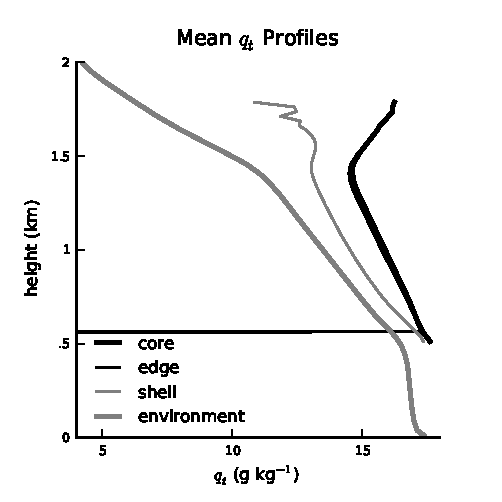
\includegraphics[width=20pc]{./figures/shell_edge_profiles_core}
  \caption{Mean profiles of $q_t$ in the cloud core (thick grey line), core 
  edge (thin black line), core shell (thin grey line), and environment (thick 
  black line).
  }
\end{figure}

\begin{figure}
  \label{fig:corrected_entrainment}
  \noindent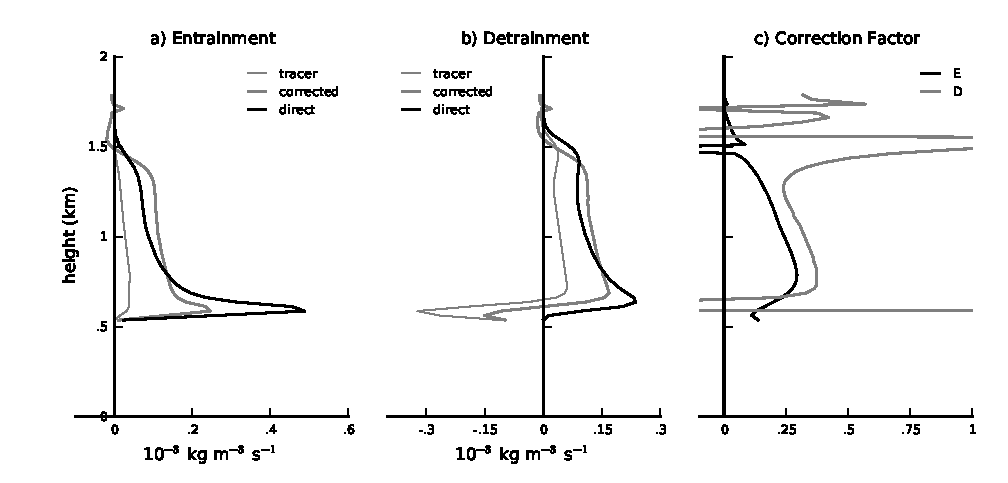
\includegraphics[width=39pc]{./figures/corrected_entrainment_core}
  \caption{Comparison of mean a) entrainment and b) detrainment profiles 
calculated using uncorrected bulk tracer budgets (thin grey line), bulk tracer 
budgets corrected for the presence of a moist cloud shell (thick grey line), and
direct flux calculations with tetrahedral surface interpolation (black line).
c) Ratio of corrected bulk tracer rates to the direct flux using
tetrahedral interpolation rates of entrainment (black) and detrainment (grey).
d) and e) are the same as a) and b) but for the fractional entrainment and
detrainment rates.}
\end{figure}

% ONE-COLUMN figure/table, including eps graphics
%
% \begin{figure}
% \noindent\includegraphics[width=20pc]{samplefigure.eps}
% \caption{Caption text here}
% \end{figure}
% \end{document}
%
% \begin{table}
% \caption{}
% \end{table}
%
% ---------------
% TWO-COLUMN figure/table
%
% \begin{figure*}
% \noindent\includegraphics[width=39pc]{samplefigure.eps}
% \caption{Caption text here}
% \end{figure*}
%
% \begin{table*}
% \caption{Caption text here}
% \end{table*}
%
% see below for how to make landscape figures or tables

%%% End the article here:

\end{document}

%%%%%%%%%%%%%%%%%%%%%%%%%%%%%%%%%%%%%%%%%%%%%%%%%%%%%%%%%%%%%%%


%% ------------------------------------------------------------------------ %%
%
%  IN-TEXT LISTS
%
%% ------------------------------------------------------------------------ %%

% Do not use bulleted lists; enumerated lists are okay.
% \begin{enumerate}
% \item
% \item
% \item
% \end{enumerate}

%% ------------------------------------------------------------------------ %%
%
%  EQUATIONS
%
%% ------------------------------------------------------------------------ %%

% Single-line equations are centered.

% Math coded inside display math mode \[ ...\]
% will not be numbered e.g.:
% \[ x^2=y^2 + z^2\]

% Math coded inside \begin{equation} and \end{equation} will
% be automatically numbered e.g.:
% \begin{equation}
% x^2=y^2 + z^2
% \end{equation}

% IF YOU HAVE MULTI-LINE EQUATIONS, PLEASE
% BREAK THE EQUATIONS INTO TWO OR MORE LINES
% OF SINGLE COLUMN WIDTH (20 pc, 8.3 cm)
% using double backslashes (\\).

% To create multiline equations, use the
% \begin{eqnarray} and \end{eqnarray} environment
% as demonstrated below.
\begin{eqnarray}
  x_{1} & = & (x - x_{0}) \cos \Theta \nonumber \\
        && + (y - y_{0}) \sin \Theta  \nonumber \\
  y_{1} & = & -(x - x_{0}) \sin \Theta \nonumber \\
        && + (y - y_{0}) \cos \Theta.
\end{eqnarray}

If you don't want an equation number, use the star form:
\begin{eqnarray*}...\end{eqnarray*}

% Break each line at a sign of operation
% (+, -, etc.) if possible, with the sign of operation
% on the new line.

% Indent second and subsequent lines to align with
% the first character following the equal sign on the
% first line.

% Use an \hspace{} command to insert horizontal space
% into your equation if necessary. Place an appropriate
% unit of measure between the curly braces, e.g.
% \hspace{1in}; you may have to experiment to achieve
% the correct amount of space.

% There is another multiline equation environment:
% \begin{aguleftmath}...\end{aguleftmath}
% The equation is aligned left and the second line indents to
% the width of a paragraph indent (AGU style)


%% ------------------------------------------------------------------------ %%
%
%  EQUATION NUMBERING: COUNTER
%
%% ------------------------------------------------------------------------ %%

% You may change equation numbering by resetting
% the equation counter or by explicitly numbering
% an equation.

% To explicitly number an equation, type \eqnum{}
% (with the desired number between the brackets)
% after the \begin{equation} or \begin{eqnarray}
% command.  The \eqnum{} command will affect only
% the equation it appears with; LaTeX will number
% any equations appearing later in the manuscript
% according to the equation counter.
%
% To reset the equation counter, place the setcounter{equation}
% command in front of your equation(s).
%\setcounter{equation}{0}

% Set the equation counter to 0 if the next
% number needed is 1 or set it to 7 if the
% next number needed is 8, etc.
%
% The \setcounter{equation} command does affect
% equations appearing later in the manuscript.

% If you have a multiline equation that needs only
% one equation number, use a \nonumber command in
% front of the double backslashes (\\) as shown in
% the multiline equation above.



%%%%%%%%%%%%%%%%%%%%%%%%%%%%%%%%%%%%%%%%%%%%%%%%%%%%%%
%% Landscape figure and table examples
%
% ---------------
% Landscape (broadside) figure/table
% (These objects will not display properly in draft mode, use galley.)
%
% ONE-COLUMN landscape figure and table
%
% \begin{landscapefigure}
% \includegraphics[height=.75\mycolumnwidth,width=42pc]{samplefigure.eps}
% \caption{Caption text here}
% \end{landscapefigure}
%
% \begin{landscapetable}
% \caption{Caption text here}
% \begin{tabular*}{\hsize}{@{\extracolsep{\fill}}lcccc}
% \tableline
% ....
% \tableline\\
% \multicolumn5l{(a) Algorithms from Numerical Recipes}\\
% \end{tabular*}
% \tablenotetext{}{}
% \tablecomments{}
% \end{landscapetable}
%
% FULL-PAGE landscape figures and tables
%
% \begin{figure*}[p]
% \begin{landscapefigure*}
% illustration here
% \caption{caption here}
% \end{landscapefigure*}
% \end{figure*}
%
% \begin{table}[p]
% \begin{landscapetable*}
% \caption{}
% \begin{tabular*}{\textheight}{@{\extracolsep{\fill}}lccrrrcrrr}
% ....
% \end{tabular*}
% \begin{tablenotes}
% ...
% \end{tablenotes}
% \end{landscapetable*}
% \end{table}
%
